\chapter{Design Details for Evolution Scenarios}
In this chapter we provide the detailed design documentation for each of the evolution scenarios
introduced in the prior section. Sec. \ref{App} sketches the design decision for the Mobile App that provides a second sales channel next to the existing Pick-up Shop. Sec. \ref{Docker} describes the adaptive changes of using a Docker environment to simplify the update process. They are both based on, or at least use the Hybrid Cloud-based Variant of CoCoME \cite{HeinrichRostamiReussner2016_1000052688}. In contrast, Sec. \ref{MS} provides a detailed design documentation of a new architectural version of CoCoME. This perfective evolution scenario is realized based on the Microservice idea.

\section{Adding a Mobile App Client} \label{App}
Developing the Mobile App Client as an extension of CoCoME requires additional use cases. They are described in Sec. \ref{UseCasesMobileApp}. Sec. \ref{DesignMobileApp} describes extensions on design level. The content of this chapter mainly originates from \cite{schnabel}.
\subsection{Use Cases of the Mobile App}\label{UseCasesMobileApp}
		\begin{figure}[t]
			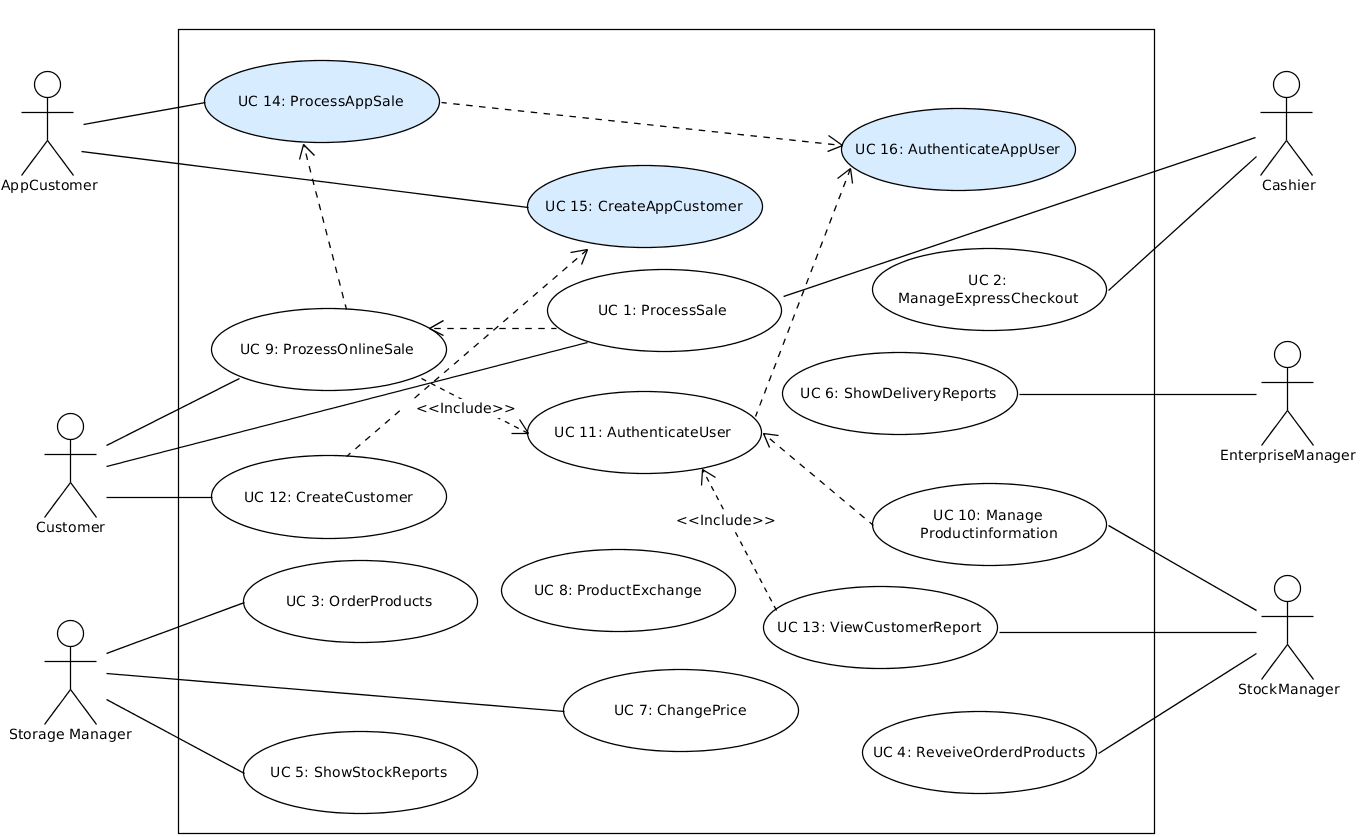
\includegraphics[width=\textwidth]{img/appUseCase.png}
			\caption{Use Case Diagram CoCoME Mobile App}
		\end{figure}

\textbf{UC 14 - ProcessAppSale}\\
\textit{Brief Description} A Customer selects the product items s/he wants to buy and the payment by credit card is performed.\\ \newline
\textit{Involved Actors} AppCustomer, Bank\\ \newline
\textit{Precondition} The App is ready to process a new sale and the Customer already has an account registered in the System.\\ \newline
\textit{Trigger} The Customer opens the app and wants to buy product items.\\ \newline
\textit{Postcondition} The Customer has paid and the sale is registered in the inventory.\\ \newline
\textit{Standard Process}
\begin{itemize}[leftmargin=*]
	\item[1.] The AppCustomer searches products provided by the App.
	\item[2.] The AppCustomer can see details for each product on a separate site.
	\item[3.] The AppCustomer adds the product items s/he wants to purchase to the Shopping Cart. Step 1-3 is repeated until all items are added to the cart.
	\item[4.] The AppCustomer gets an overview of the items in the cart, their price and the running total.
	\item[5.] The AppCustomer proceed to the Checkout 
	\item[6.] The AppCustomer selects the Store where s/he wants to pick up his/her	purchased product items. 
	\item[7.] The AppCustomer is presented with a login form and is required to complete the "Authenticate user" use case.
	\item[8.] In order to initiate card payment, the customer selects a credit card used for the purchase.
	\item[9.] The AppCustomer enters his/her PIN in the designated field presented by the System.
	\item[10.] The System presents the Customer with an overview of the purchase, the AppCustomer confirms the purchase and waits for validation. Step 9 is repeated until the validation is successful or the Customer decides to cancel the purchase.
	\item[11.] Completed sales are logged by the System and sale information are sent to	the Inventory in order to update the stock.
	\item[12.] A success message is presented to the AppCustomer and the product items
	are being prepared to be picked up by the customer.
	\item[13.] The AppCustomer closes the app.
\end{itemize}

\textit{Alternative or Exceptional Processes}
\begin{itemize}
	\item[-] In step 8: No Card available
	\begin{itemize}
		\item[1.] In order to add a new credit card the Customer clicks the Add Card button.
		\item[2.] The Customer enters the card number of the new credit card and saves the card.
	\end{itemize}
	
	\item[-] In step 10: Card validation fails
	\begin{itemize}
		\item[1.] The Customer tries again and again.
		\item[2.] Otherwise, the Customer can decide to cancel the purchase.
	\end{itemize}
\end{itemize}


\textbf{UC 15 - CreateAppCustomer}\\ \newline
\textit{Brief Description} The app offers a possibility to create a new Customer account.\\ \newline
\textit{Involved Actors} AppCustomer\\ \newline
\textit{Precondition} The Customer does not have a Customer account yet and the app is started.\\ \newline
\textit{Trigger} A new AppCustomer wants to create an account.\\ \newline
\textit{Postcondition} The User is authenticated.\\ \newline
\textit{Standard Process}
\begin{itemize}[leftmargin=*]
	\item[1.] The AppCustomer has to fill out forms, requesting all necessary information to create a new AppCustomer account.
	\begin{itemize}
		\item[(a)] Form for name, email and password
		\item[(b)] Form for address
		\item[(c)] Summery of the information 
	\end{itemize}
	\item[2.]The Customer fills out the forms, verifies and submits the information.
	\item[3.] The app verifies the given information and creates a new Customer account in the Inventory.
\end{itemize}

\textit{Alternative or Exceptional Processes}
\begin{itemize}
	\item[-] In step 3 : Provided information is incorrect or not valid. The Customer is notified of the problem and enters the information again until it passes the check.	
\end{itemize}

\textbf{UC 16 - AuthenticateAppUser}\\ \newline
\textit{Brief Description} The app provides the possibility to authenticate a User.\\ \newline
\textit{Involved Actors} AppCustomer\\ \newline
\textit{Precondition} The app is started.\\ \newline
\textit{Trigger} An AppCustomer wants to authenticate his/herself.\\ \newline
\textit{Postcondition} The AppCustomer is authenticated.\\ \newline
\textit{Standard Process}
\begin{itemize}[leftmargin=*]
	\item[1.] The AppCustomer gets displayed a login form. S/he is asked to enter email and password.
	\item[2.] The App checks the provided credentials. If correct, the AppCustomer is logged in.
\end{itemize}

\textit{Alternative or Exceptional Processes}
\begin{itemize}
	\item[-] In step 2: Wrong credentials
	\begin{itemize}
		\item[1.] An error message is displayed.
		\item[2.] The User may try again until the authentication succeeds.
	\end{itemize}
\end{itemize}


\newpage

\subsection{Design of the Mobile App}\label{DesignMobileApp}
 Fig. \ref{ComponentApp} is the component of this evolution scenario. When adding the Mobile App client, the hybrid cloud-based variant of CoCoME did not have to be modified. Therefore, CoCoME is encapsulated in a single component. Simply the three web services \textit{WebService::Inventory::LoginManager, WebService::Inventory::Store and WebService::Inventory::Enterprise} used by the App Client are emphasized. The entire component diagram for the hybrid cloud-based variant is available in the Technical Report \cite{HeinrichRostamiReussner2016_1000052688}. 
 \\ Fig. \ref{ComponentApp} indicates that the AppShop requires an adapter to access the web services provided by CoCoME. This is because CoCoME uses SOAP/WS*-based web services which are not compatible with the technology used to implement the AppShop Client. A more detailed introduction about the technology used to implement the Mobile App Client can be found in \cite{schnabel}. 
  
 \begin{figure}[!h]
	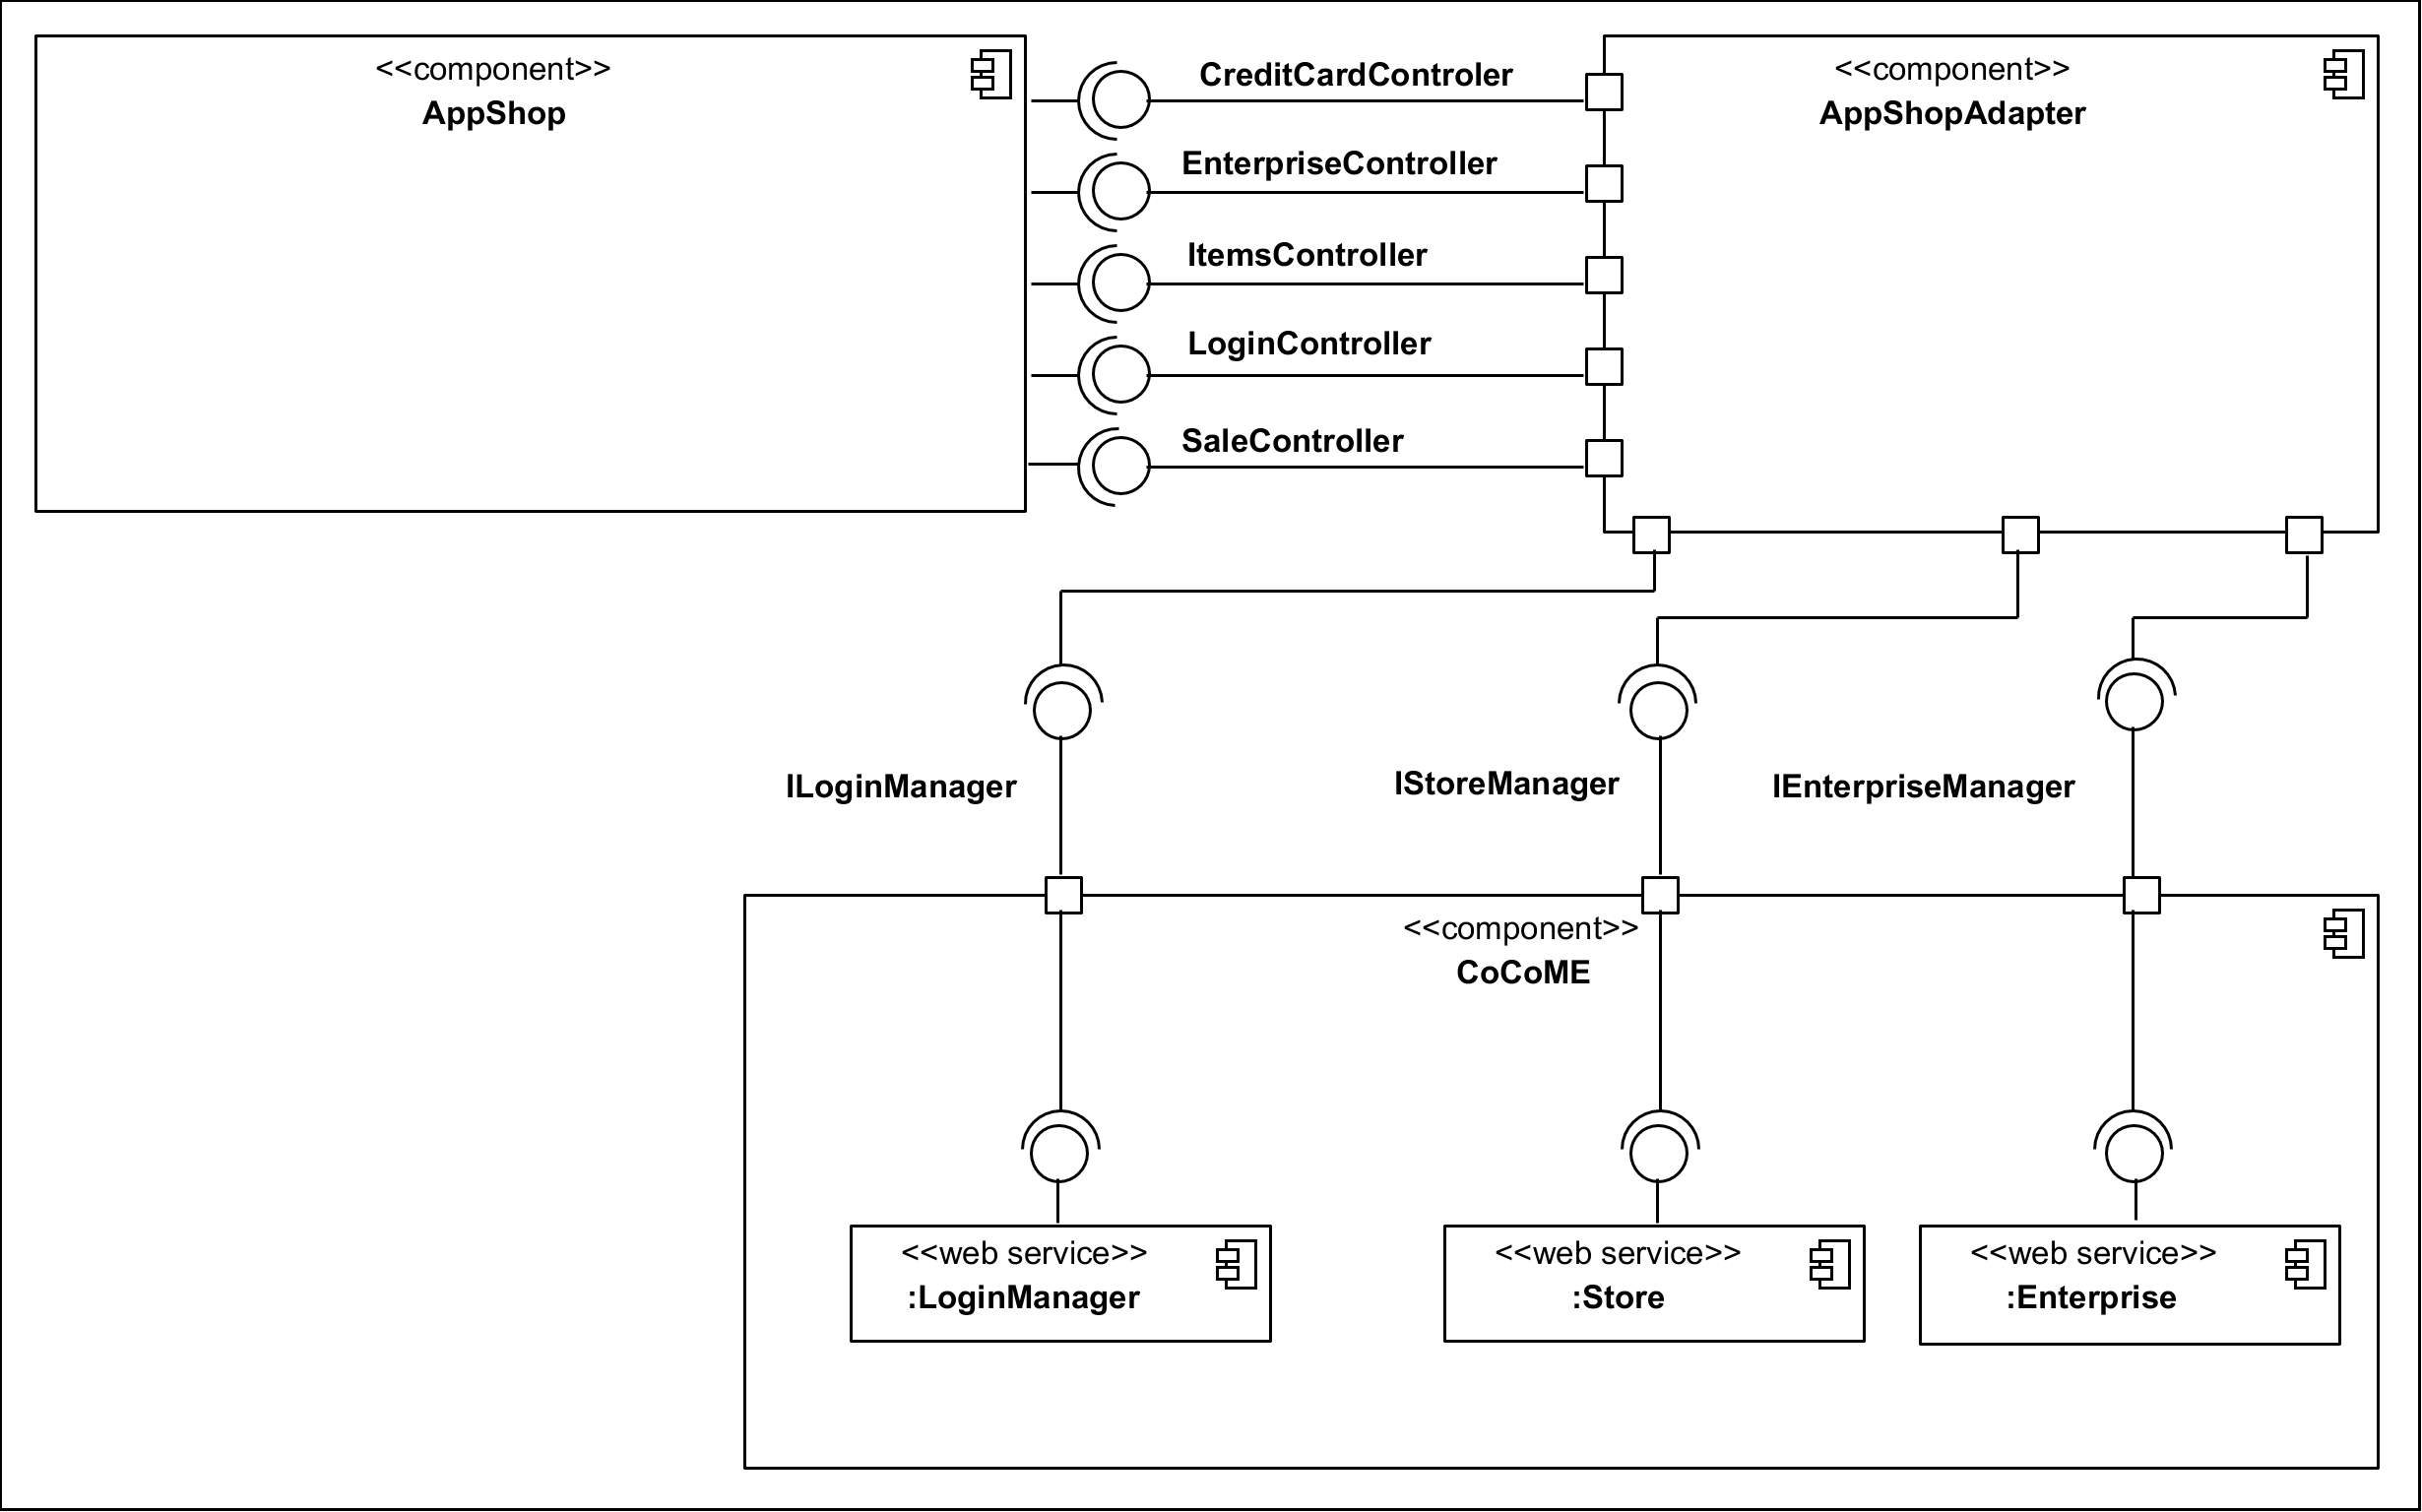
\includegraphics[width=\textwidth]{img/appComponent.png}
	\caption{Component Diagram of the CoCoME Ecosystem After Adding the Mobile App Client}
	\label{ComponentApp}
\end{figure}

  The \textit{AppShopAdapter} consumes the three web services \textit{WebService::Inventory::LoginManager, WebService::Inventory::Store} and \textit{WebService::Inventory::Enterprise} and provides a Rest Api which is used by the actual \textit{AppShop}. The Rest Api contains endpoints to retrieve and process Credit Card, Enterprise and StockItem information. To implement \emph{UC14-16}, the Api also provides endpoints for user management and processing sales. 
  
\begin{figure}[!h]
	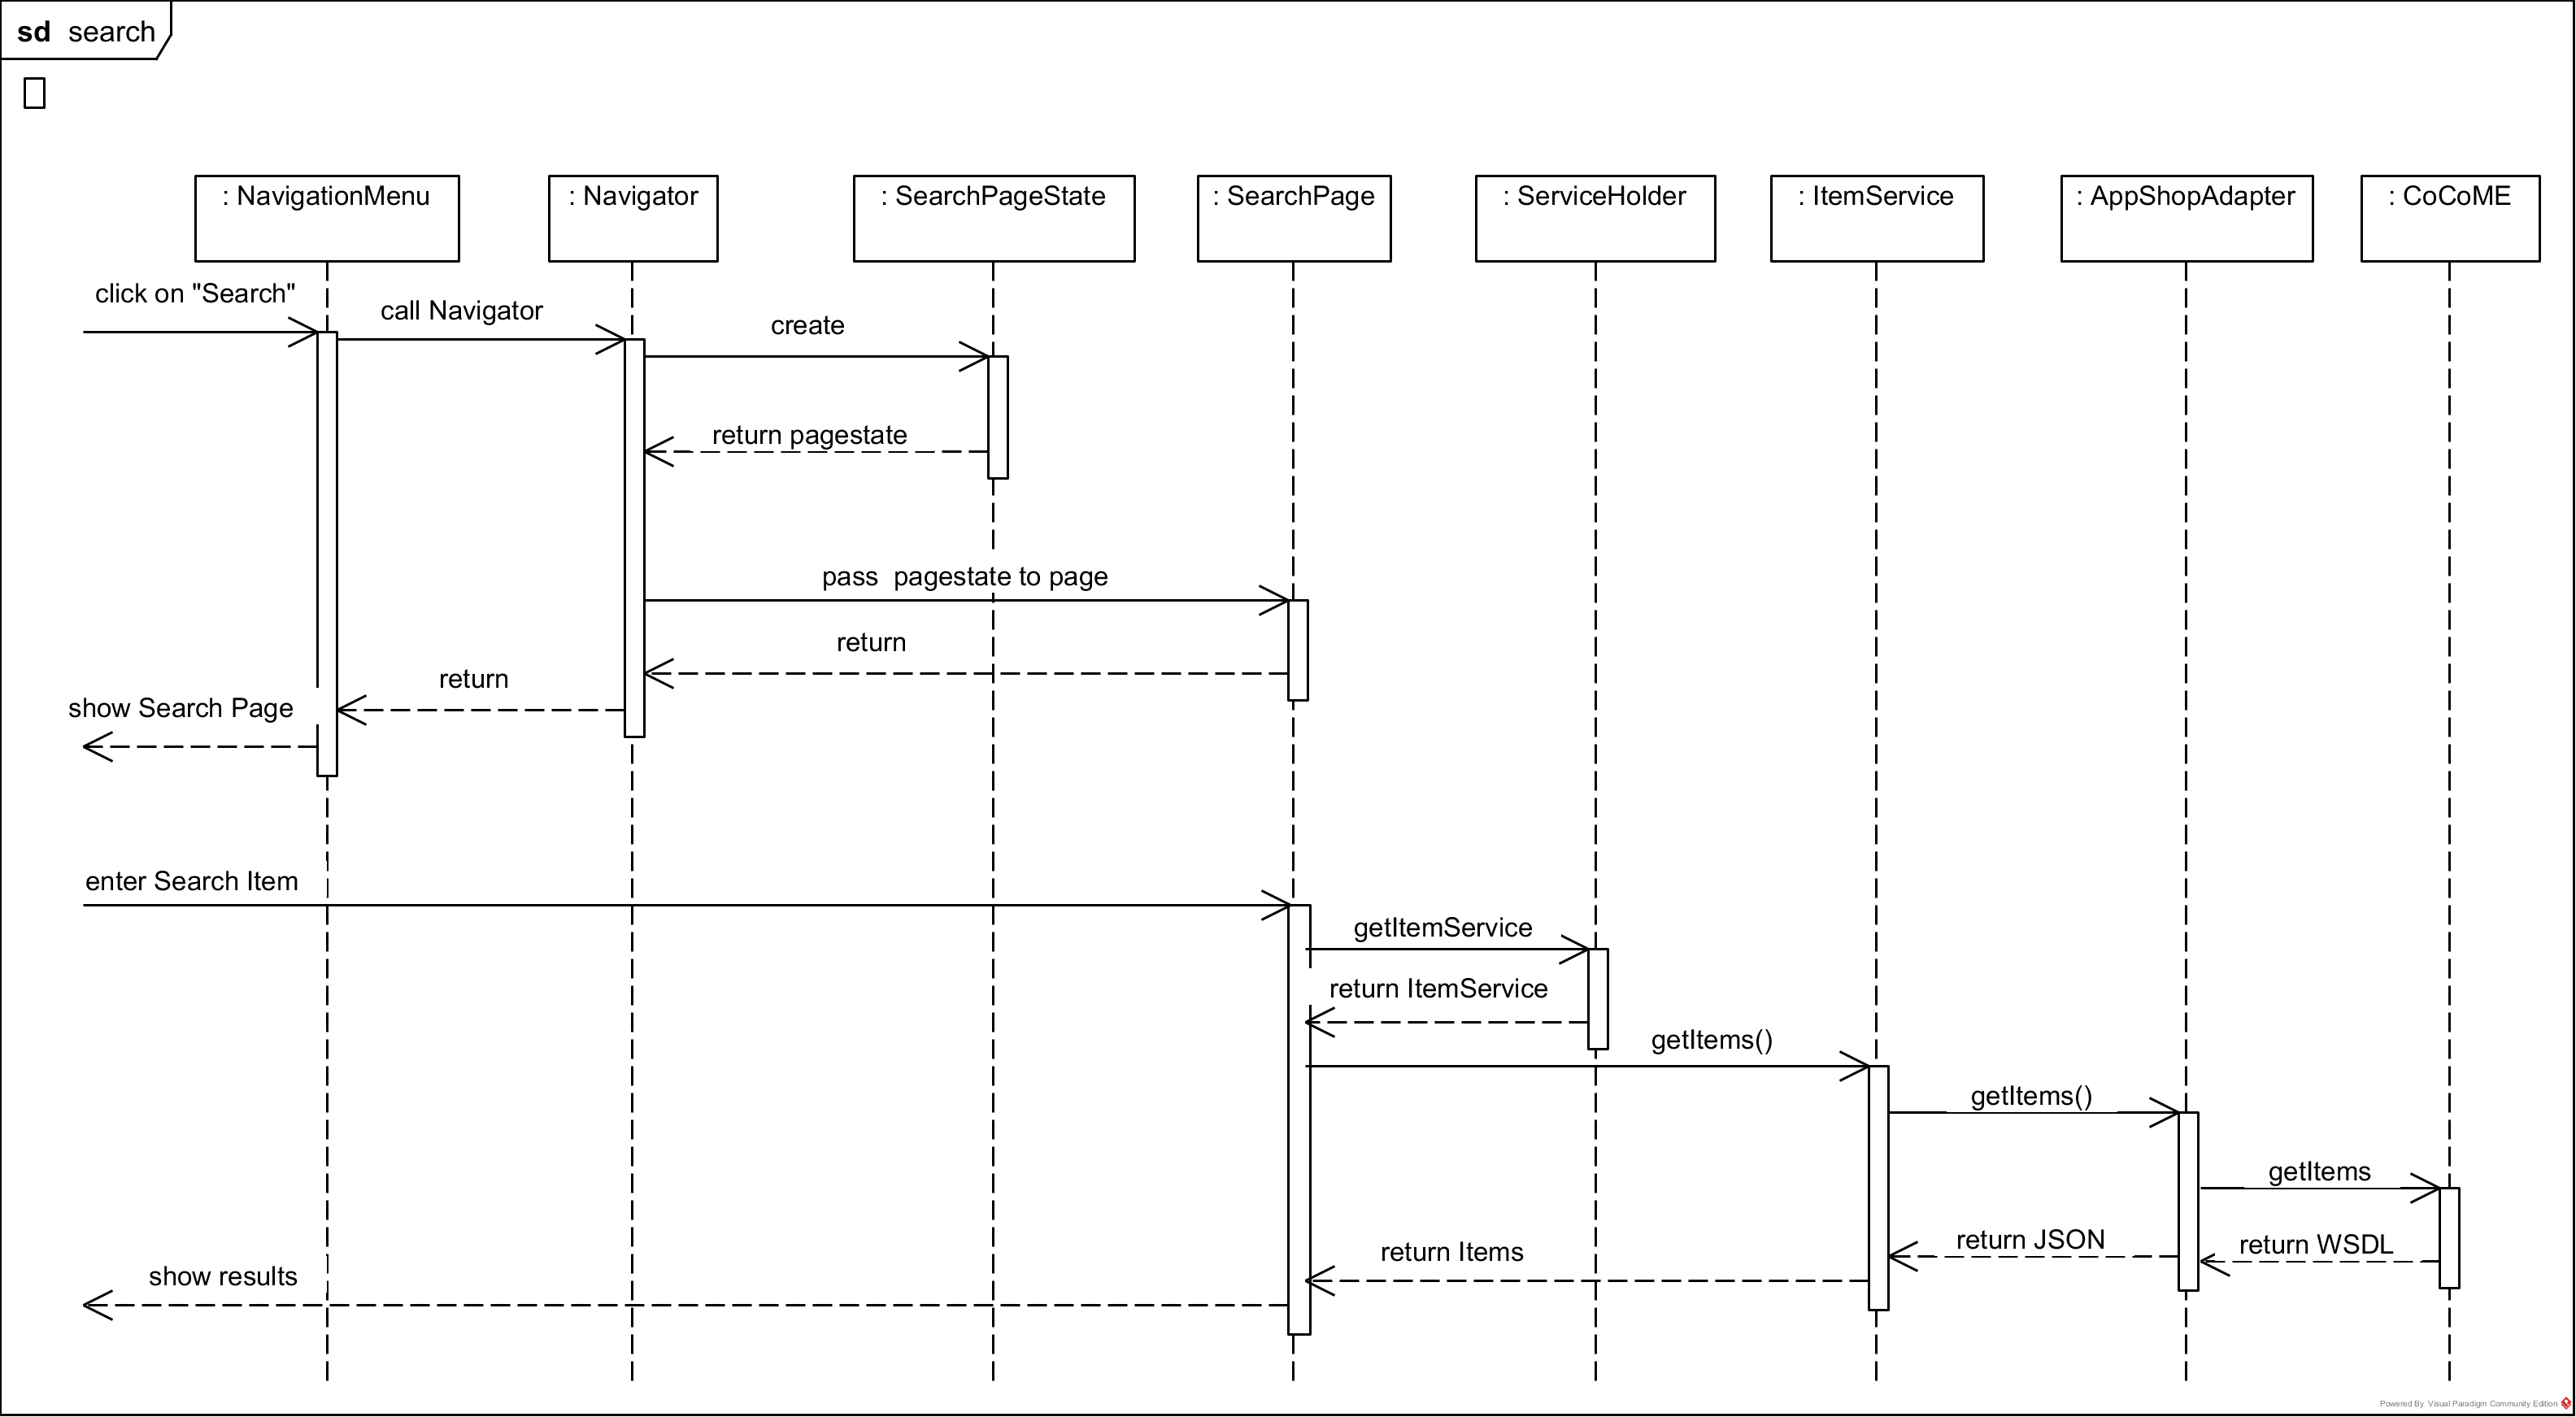
\includegraphics[width=\textwidth]{img/appSearchSequence.png}
	\caption{Sequence Diagram of Searching an Item in the Mobile App Client}
	\label{SequenceAppSearch}
\end{figure}

Fig. \ref{SequenceAppSearch} shows the process of opening a page to search for an Item. The customer opens the \textit{WebShopClient} and triggers the "Search" function to search for an item. To open the page, the \textit{NavigatorMenu} must call the \textit{Navigator} which creates a pagestate object and passes the object to the page. This HTML page is now presented to the customer. To fill the page with information, i.e when searching for a \textit{ProductItem}, the page uses services provided by the \textit{ServiceHolder}. In this case, the \textit{ItemService} calls the responsible REST-Service of \textit{AppShopAdapter} which in turn retrieves the necessary information from the WSDL services provided by CoCoME.


Fig. \ref{SequenceAppSale} demonstrates how the Mobile App Client processes sales.  For the sake of clarity, the digram is simplified and only contains the most important calls. First, the customer searches for items (according to Fig. \ref{SequenceAppSearch}). By clicking on the desired Item, the according \textit{ItemPage} is shown. This page carries information about the Item. Here, the customer decides whether the Item should be added to the Shopping Cart or not. The last steps are repeated until the customer decides to proceed to the checkout. If not logged in, the customer gets forwarded to the \textit{LoginPage}. When successfully logged in, the customer clicks the \textit{BuyNow}-Button. The Sale process is finished as soon as the backend (CoCoME) has processed the sale.




\begin{figure}[!h]
	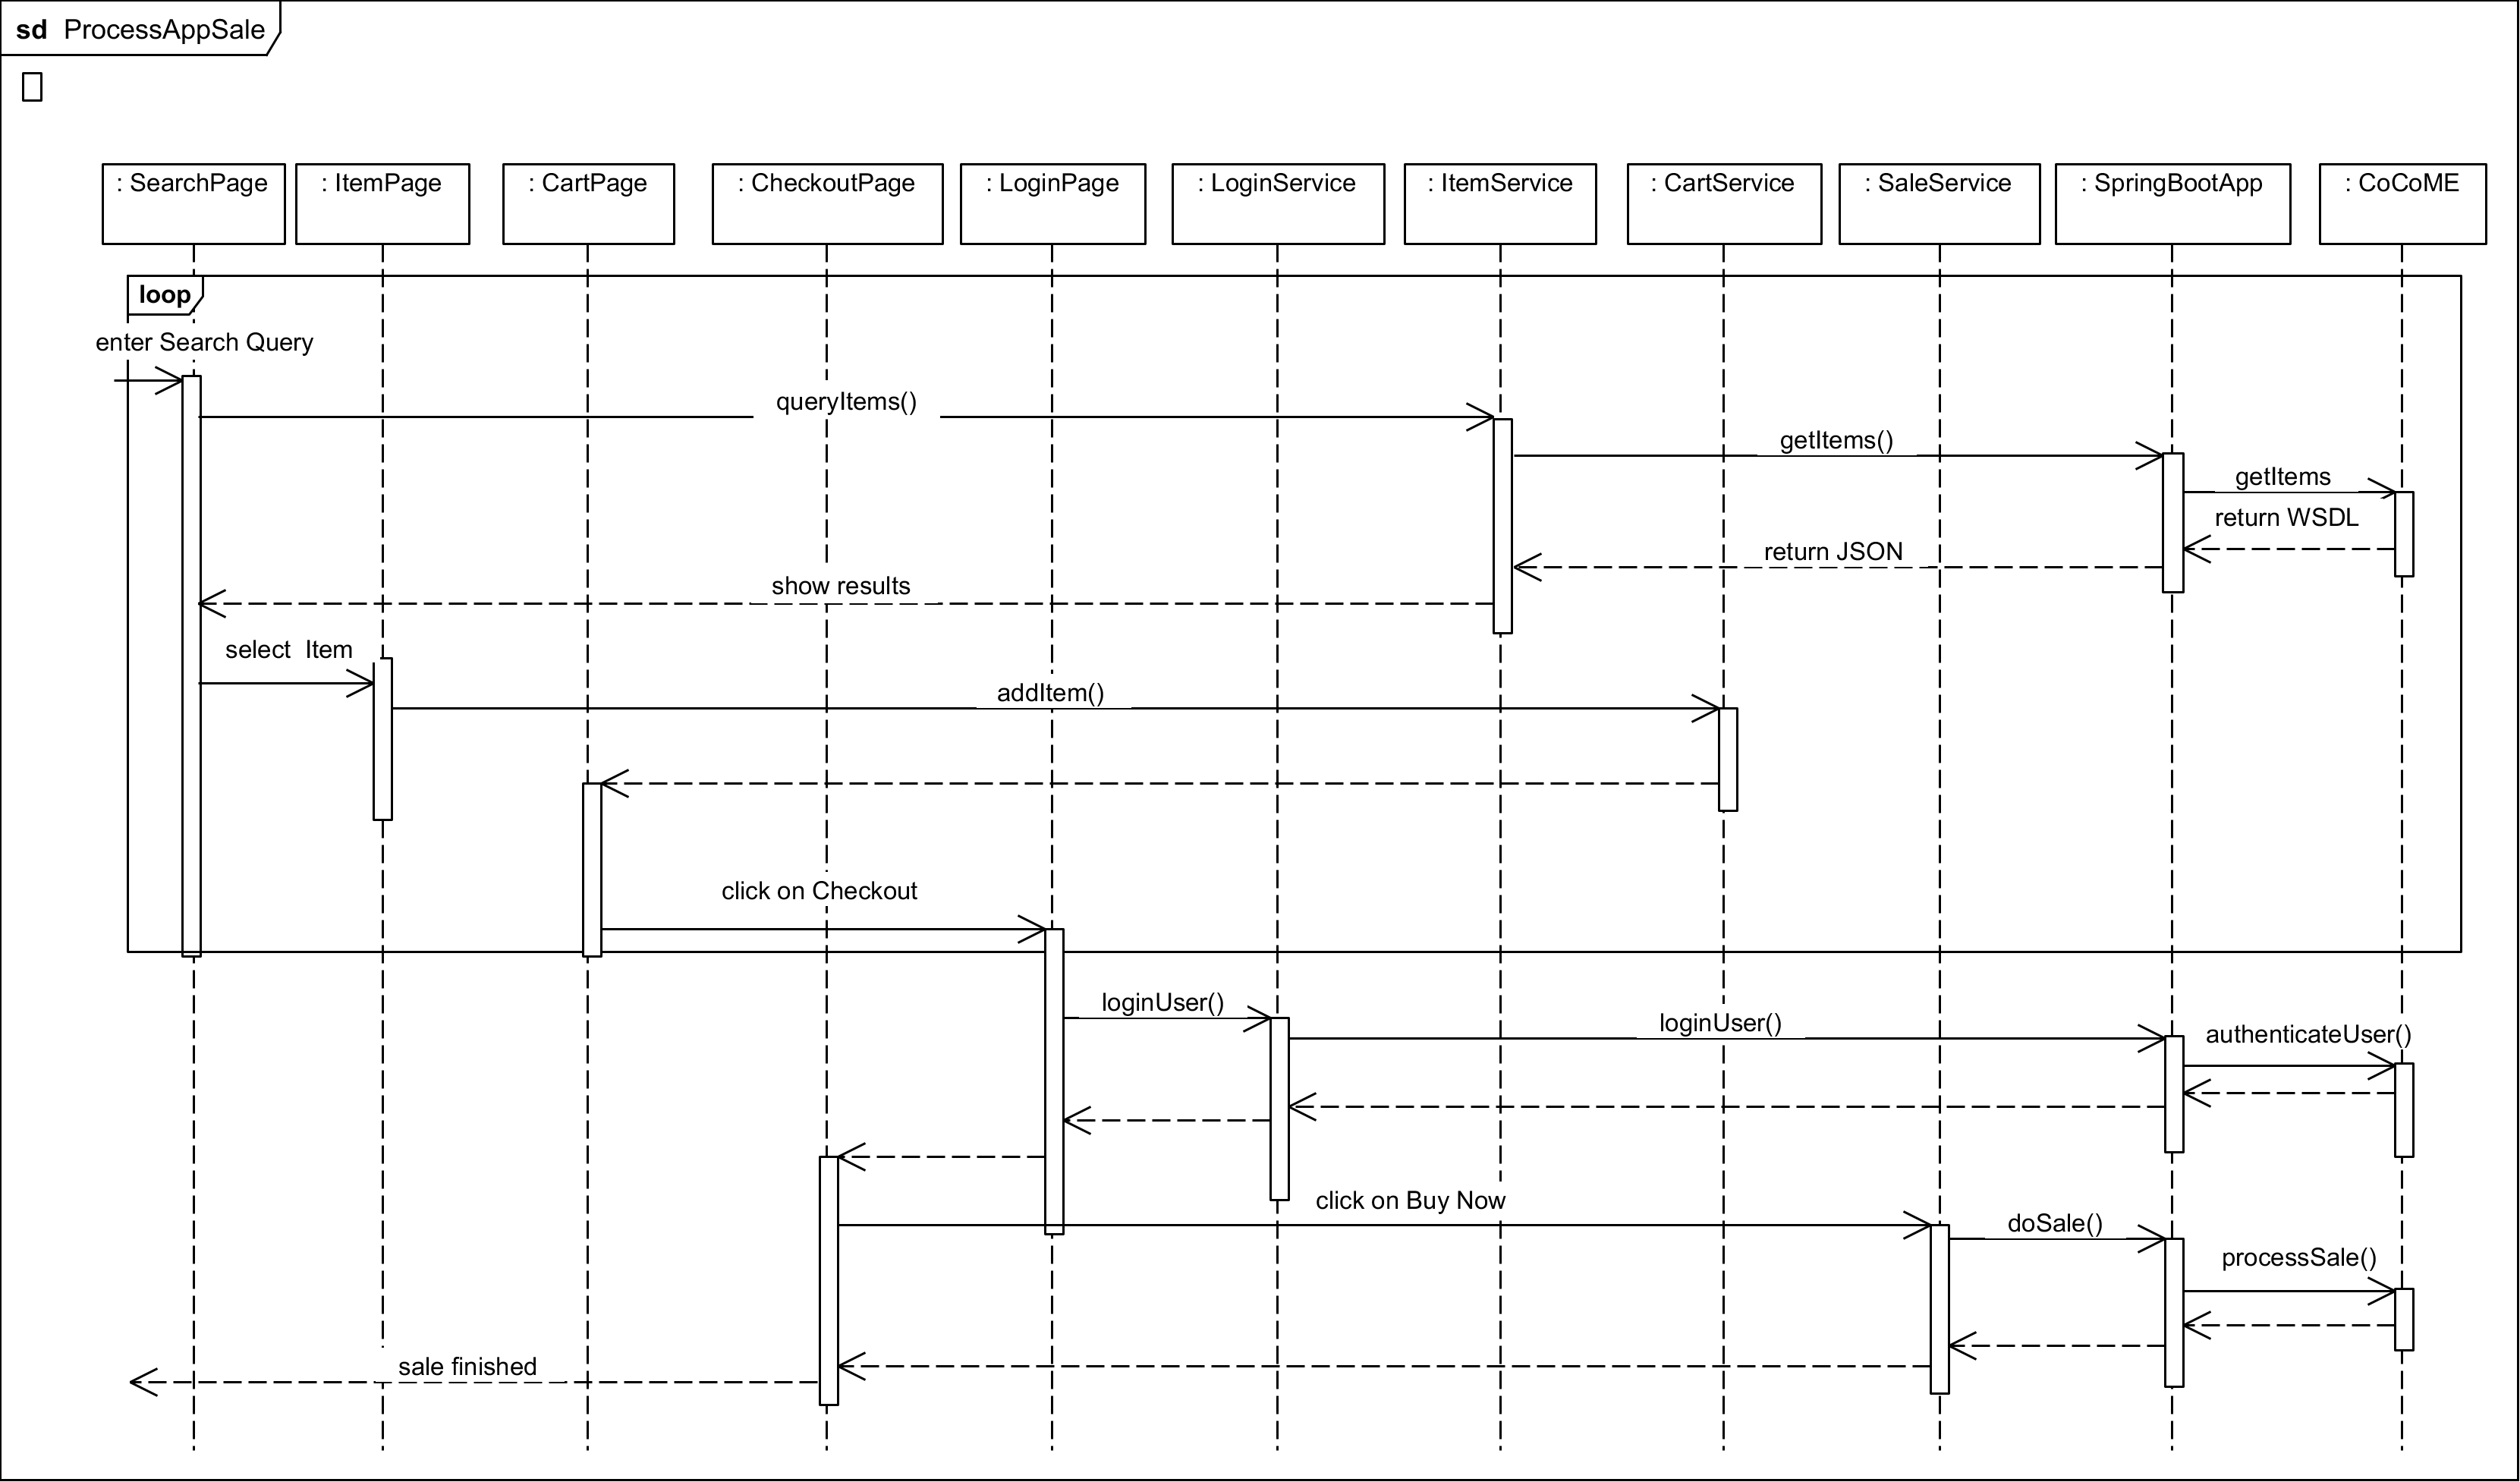
\includegraphics[width=\textwidth]{img/appProcessSale.png}
	\caption{Sequence Diagram of Processing a Sale}
	\label{SequenceAppSale}
\end{figure}

\newpage

\section{Using a Docker Environment} \label{Docker}

As shown in Fig. \ref{techStack}, using a Docker Environment affects the technology stack by adding additional layers. More detailed, the given CoCoME Stack is moved into the Docker Deamon, which runs a Linux distribution.The original parts of the stack, like Glassfish and the Java Virtual Machine, are still a part of the stack.
	
	\begin{figure}[!h]
		\centering
		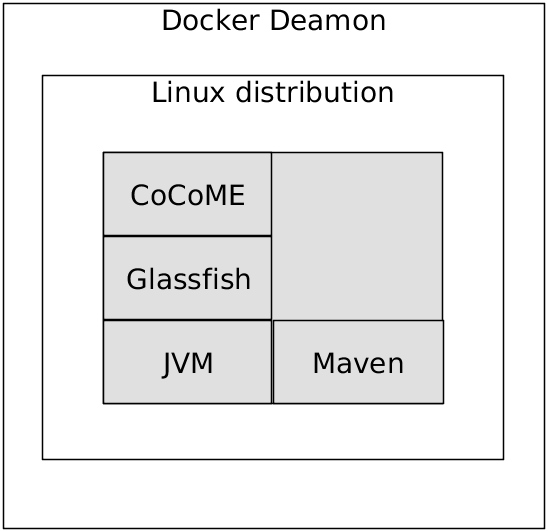
\includegraphics[width = 0.5\textwidth]{img/tech_stack_CoCoME.png}
		\caption{Extended technology stack CoCoME}
		\label{techStack}
	\end{figure}
	
The Dockerfile defines an environment based on the latest version of Ubuntu 16:04. Maven, Git and Java are also installed using the standard Ubuntu package manager.\\
Git has two purposes: On the one hand it is used to download the most recent version of CoCoME.	On the other hand, it is used to download a prefabricated version of Glassfish that already includes domains and other adjustments required for CoCoME. Java is required by Glassfish and CoCoME as they need the Java Virtual Machine. Maven is needed to deploy the latest version of CoCoME onto the provided Glassfish servers.
	
	
	During the development, it was decided to implement and provide two different versions. The first version always pulls the most recent CoCoME source code from GitHub, downloads the entire dependencies with Maven, compiles and builds the project and finally deploys CoCoME on the Glassfish servers. As a consequence, creating and starting a Docker Container takes about one hour.\\
	In contrast, the second version only pulls a prefabricated version of CoCoME from GitHub. 
	Therefore, pulling the source code up to building the project is skipped. Maven does not have to be included in the technology stack. Solely, deploying CoCoME on the Glassfish server is necessary.\\
	This reduces the deployment time to a few minutes but has a disadvantage: The prefabricated version is updated manually. Therefore, it is sometime not the most recent version.\\
	By providing both, a fast deploying version and a current version, the user can choose what's the best for its situation.
	

	

	
\section{Microservices Technology} \label{MS}
	This section describes how the implementation of the usecases which are also implemented in the basic CoCoME version but also the general system design and the interaction of the microservices. In the following subsection \nameref{UsecaseSection} the realization details of different usecases is explained in detail. Further, the different usecases are allocated in the of the corresponding microservice. In the second subsection, named \nameref{archiOverviewMicro} the general architectural overview of the microservices is described.
	
	\subsection{Usecase implementation}\label{UsecaseSection}
	\FloatBarrier
		\subsubsection{Orders}
		This section describes the desgin of the \textit{Orders} microservice, which provides the main functionality for usecase 3 and usecase 4.\\
		
		\textbf{Behavioral View on UC 3 - Order Products} \\
		As shown in figure \ref{MS_UC3_1} and figure \ref{MS_UC3_2} this usecase is divided into two steps in the first step, user the frontend to create new OrderEntry elements. This elements are representing the different product entries at an order. It contains the informations about an the product to order and the ordering amount. They are saved in the Database until they are needed again in the second step again. 
		In the second step, the ProductOrder element is created. This Object represents the order itself, in detail information about the ordering store, the date on which this order is submitted and a collection with the OrderEntry objects of the products which are ordered in this order. Also it set in the OrderEntry objects an reference to this ProductOrder object.
		
			\begin{figure}[!h]
				\centering
				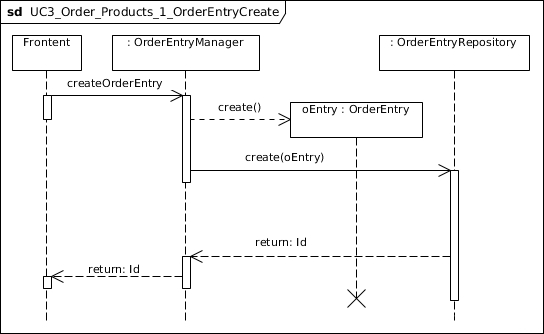
\includegraphics[width = 0.7\textwidth]{img/UC3_Order_Products_1_OrderEntryCreate.jpg}
				\caption{Usecase 3 order products, part 1}
				\label{MS_UC3_1}
			\end{figure}
			
			\begin{figure}[!h]
				\centering
				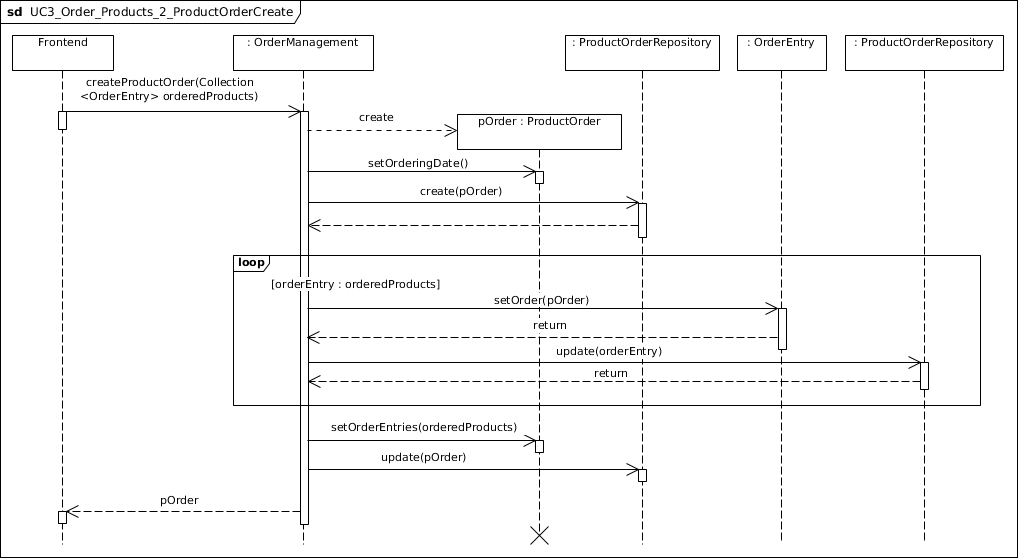
\includegraphics[width = 1\textwidth]{img/UC3_Order_Products_2_ProductOrderCreate.jpg}
				\caption{Usecase 3 order products, part 2}
				\label{MS_UC3_2}
			\end{figure}
		
		\textbf{Behavioral View on UC 4 - Receive Ordered Products} \\
		The figure %TD paste image with reference
		shows, the microservice first refreshes the store ProductOrder element and sets it delivery date to the in the call passed date.
		After this, it performs for each in the assigned a rest call to the store microservice in which the store itself is stored. With that rest call, the stockitems which are representing the corresponding product in the store are increasing their available amount of the product.
		
			
		\FloatBarrier
			
		\subsubsection{Stores}
		
			\begin{figure}[!h]
				\centering
				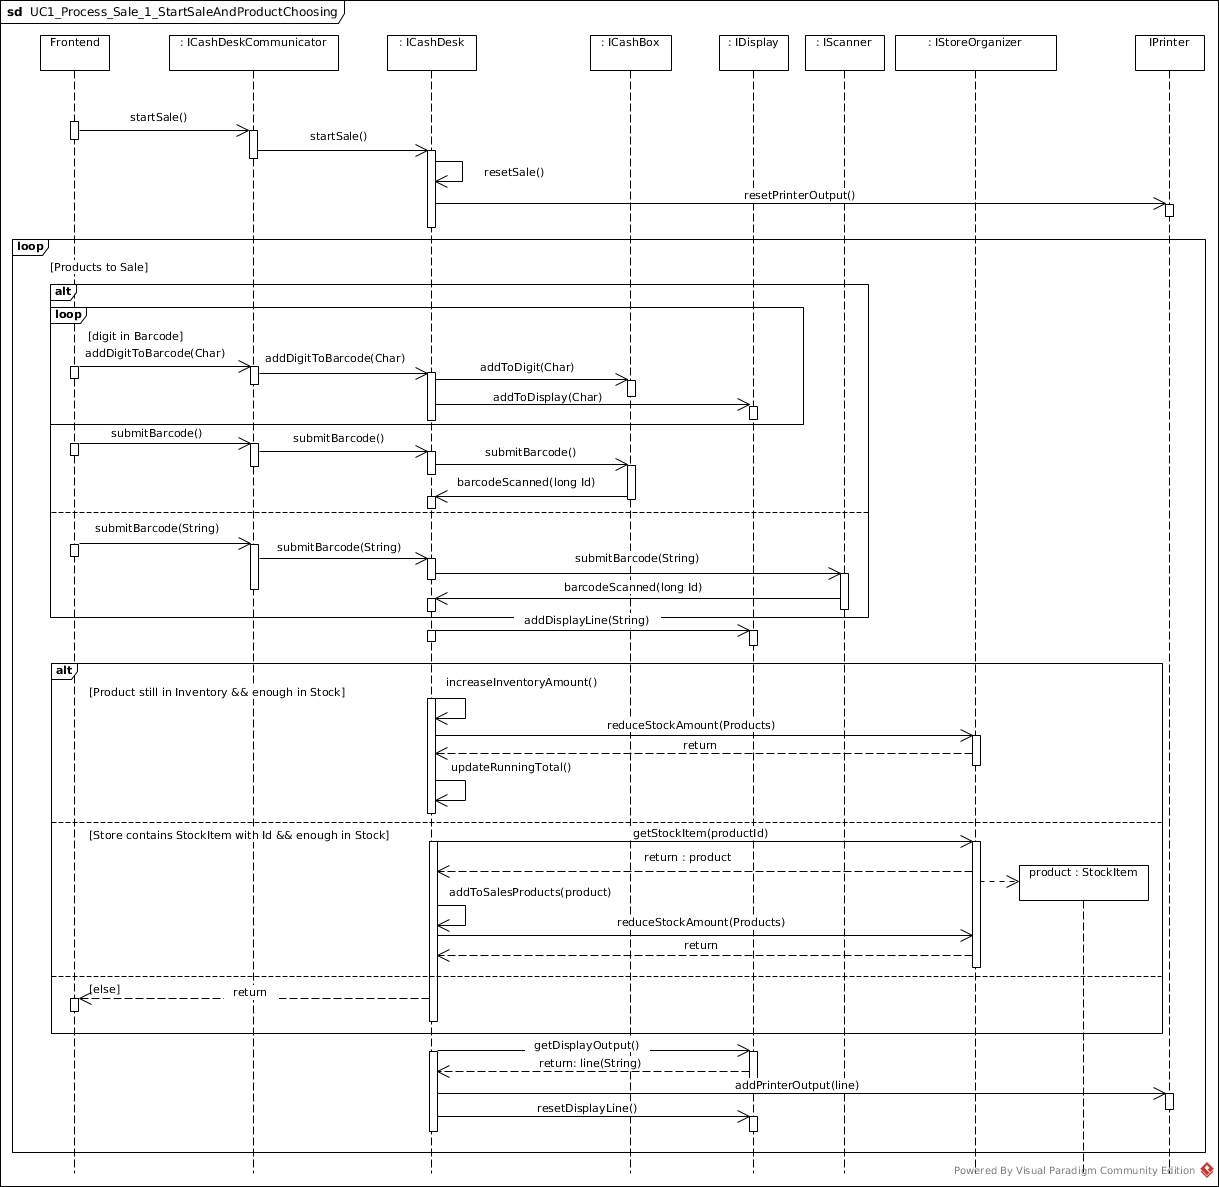
\includegraphics[width = 1\textwidth]{img/UC1_Process_Sale_1_StartSaleAndProductChoosing.jpg}
				\caption{Usecase 1 process sale, part 1}
				\label{MS_UC1_1}
			\end{figure}
			
			\begin{figure}[!h]
				\centering
				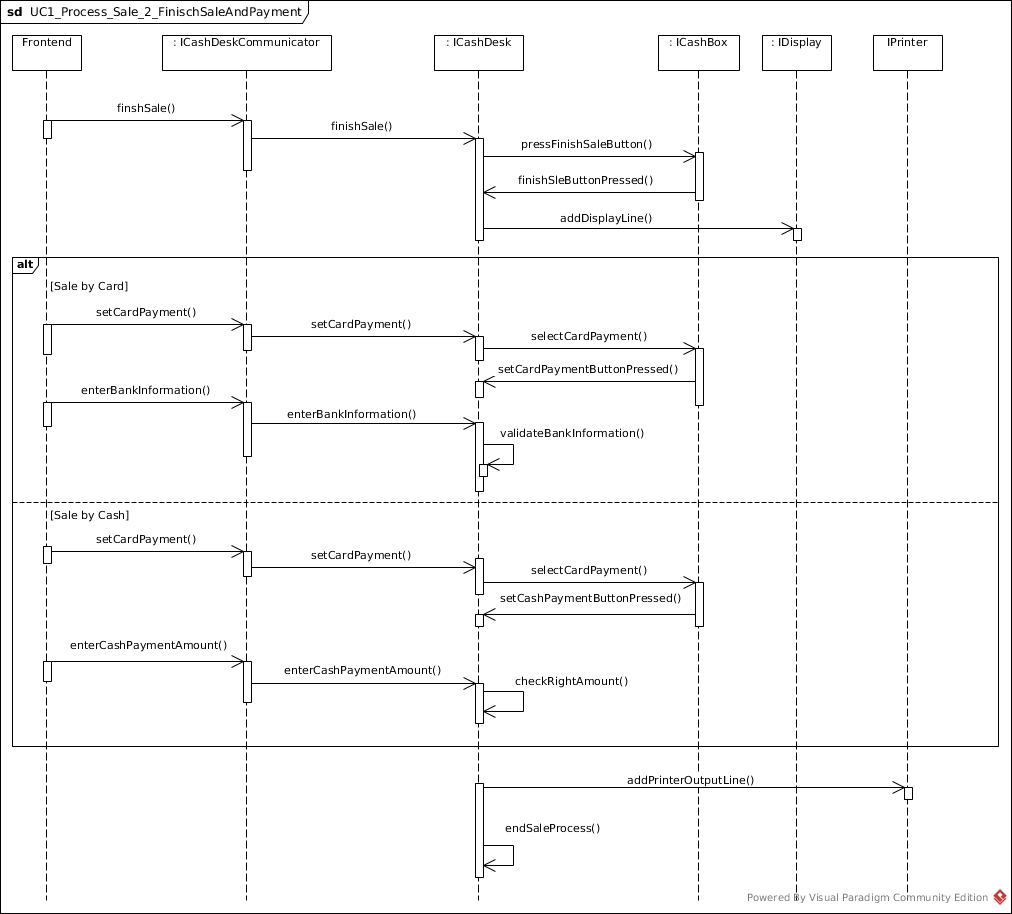
\includegraphics[width = 1\textwidth]{img/UC1_Process_Sale_2_FinishSaleAndPayment.jpg}
				\caption{Usecase 1 process sale, part 2}
				\label{MS_UC1_2}
			\end{figure}
			
			\begin{figure}[!h]
				\centering
				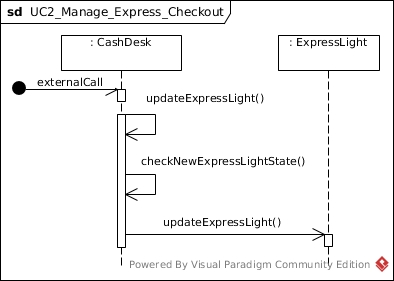
\includegraphics[width = 0.5\textwidth]{img/UC2_Manage_Express_Checkout.jpg}
				\caption{Usecase 2 manage express mode}
				\label{MS_UC2}
			\end{figure}
			
			\begin{figure}[!h]
				\centering
				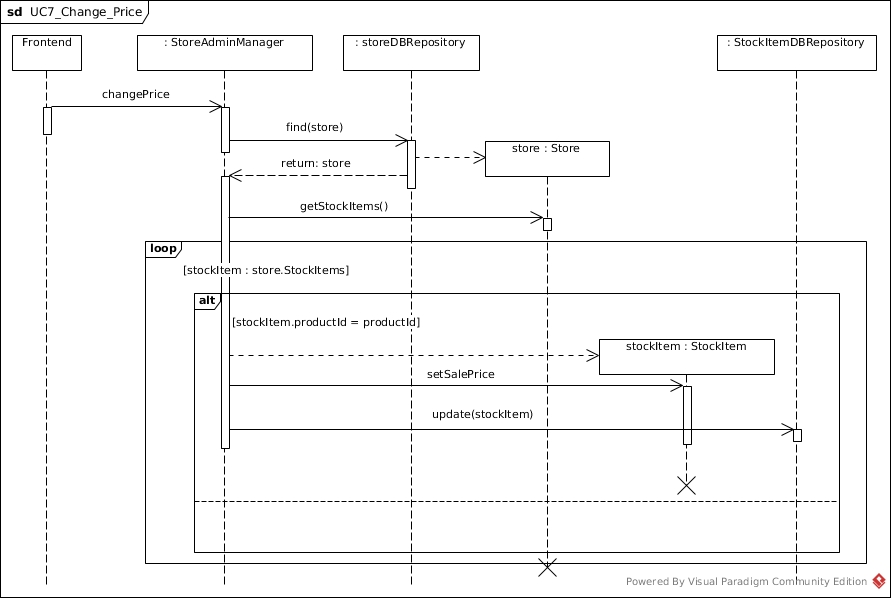
\includegraphics[width = 0.9\textwidth]{img/UC7_Change_Price.jpg}
				\caption{Usecase 7 change price}
				\label{MS_UC7}
			\end{figure}
			
			\begin{figure}[!h]
				\centering
				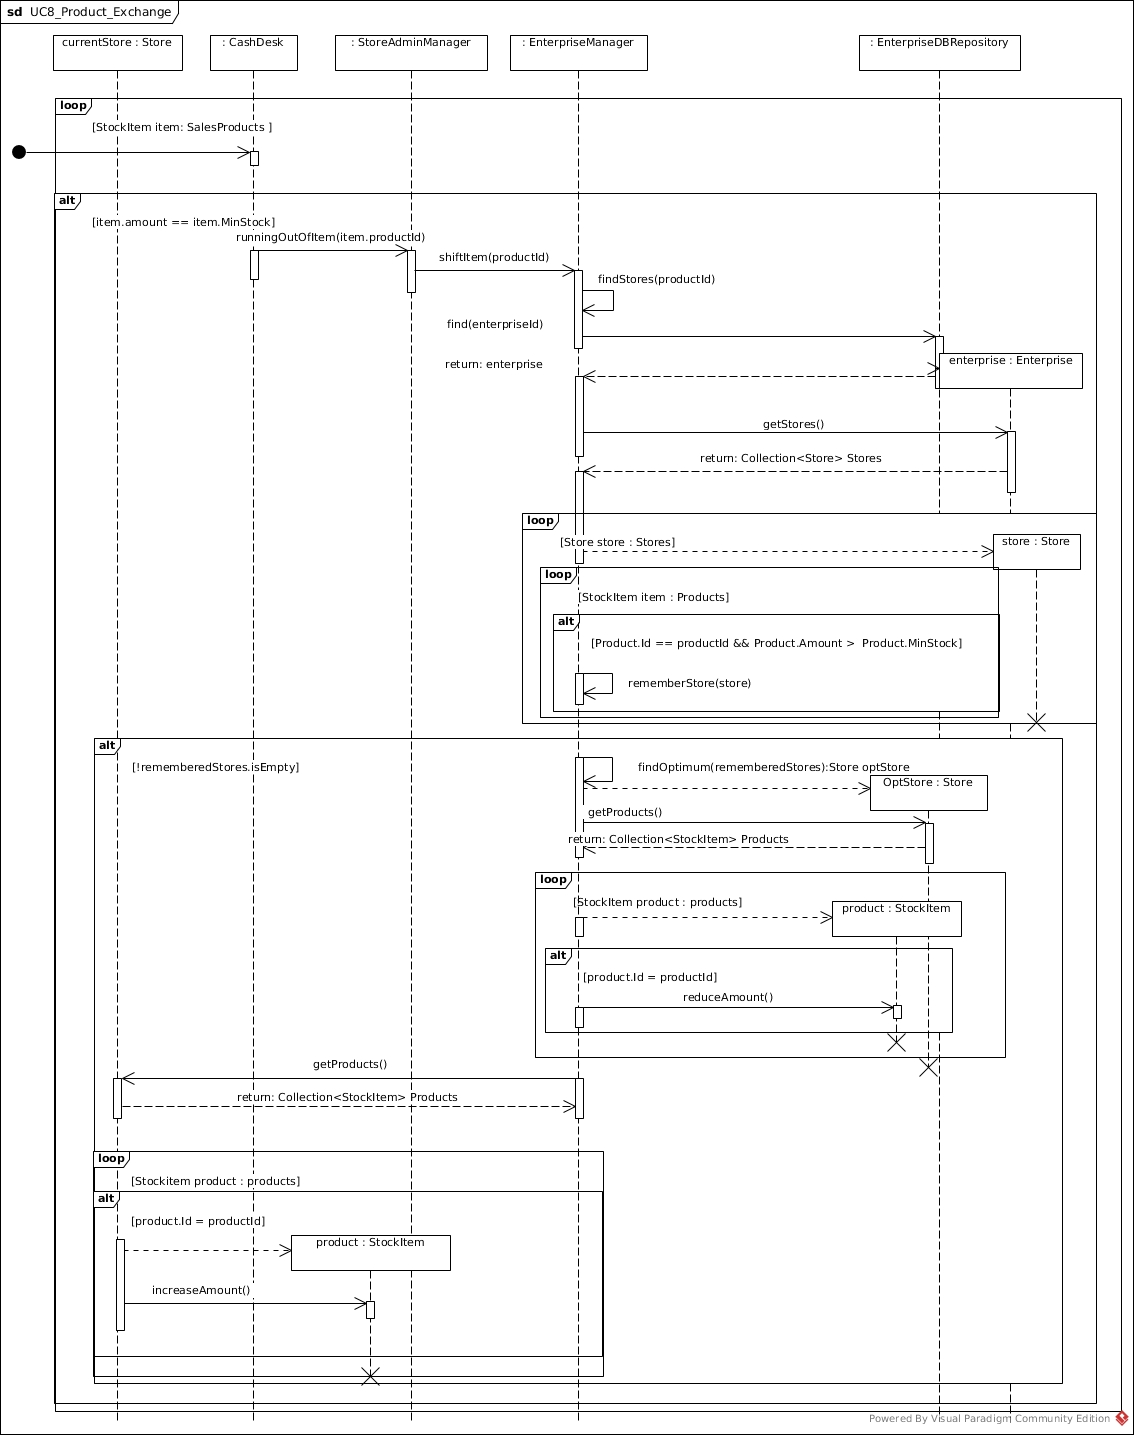
\includegraphics[width = 1\textwidth]{img/UC8_Product_Exchange.jpg}
				\caption{Usecase 8 product exchange}
				\label{MS_UC8}
			\end{figure}
		\FloatBarrier	
		
		\subsubsection{Reports}
			
			\begin{figure}[!h]
				\centering
				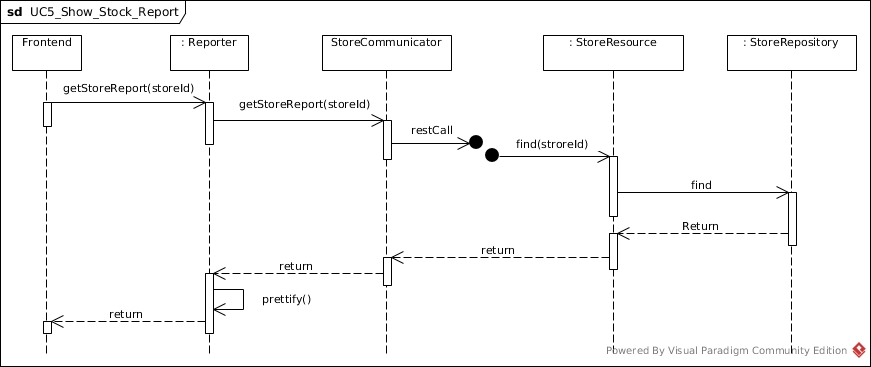
\includegraphics[width = 1\textwidth]{img/UC5_Show_Stock_Report.jpg}
				\caption{Usecase 5 show stock report}
				\label{MS_UC5}
			\end{figure}
			
			\begin{figure}[!h]
				\centering
				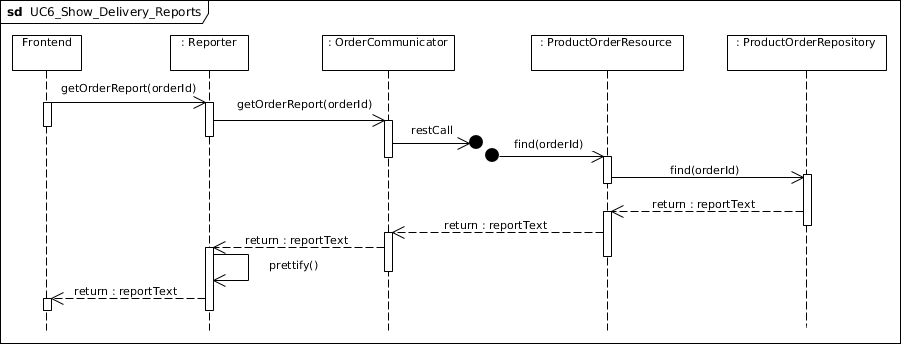
\includegraphics[width = 1\textwidth]{img/UC6_Show_Delivery_Reports.jpg}
				\caption{Usecase 6 show delivery report}
				\label{MS_UC6}
			\end{figure}
			
	\FloatBarrier
	\subsection{Architectural overview}	\label{archiOverviewMicro}	
			
